% !Mode:: "TeX:UTF-8"
% !TeX encoding = UTF-8
% !TEX program = pdflatex

\documentclass{mcmthesis}
%\usepackage[UTF8]{CTEX}

%\usepackage{fontspec,xltxtra,xunicode}
%\usepackage[slantfont,boldfont]{xeCJK}
%\setCJKmainfont[BoldFont=Adobe Heiti Std,ItalicFont=Adobe Kaiti Std]{Adobe Song Std}
%\setCJKsansfont{Adobe Heiti Std}
%\setCJKmonofont{Adobe Song Std}

\mcmsetup{CTeX = false,   % 使用 CTeX 套装时,设置为 true
	tcn = {\color{red}67859}, problem = {\color{red}D}
%	        }
	,
	sheet = false, titleinsheet = false, keywordsinsheet = false,
	titlepage = false, abstract = false}
\usepackage{palatino}
\usepackage{enumitem} % Required for manipulating the whitespace between and within lists
\usepackage{listings}
\usepackage{multirow}
\usepackage{nicefrac}
\usepackage{sectsty}
\sectionfont{\color{MidnightBlue}\selectfont}
\subsectionfont{\color{MidnightBlue!50!RoyalBlue}\selectfont}
\subsubsectionfont{\color{SkyBlue!5!RoyalBlue}\selectfont}
\usepackage{booktabs}
\usepackage{pgf}
\usepackage{tikz}
\usetikzlibrary{arrows,automata}
\usepackage{varioref} % More descriptive referencing
%\setlength\parindent{0pt}
\usepackage{subfig}
\usepackage{tikz}
\usetikzlibrary{decorations.pathmorphing} % noisy shapes
\usetikzlibrary{fit}					% fitting shapes to coordinates
\usetikzlibrary{backgrounds}	% drawing the background after the foreground
\usepackage[subfigure]{tocloft}
\renewcommand\cftsecfont{\bfseries\textbf{\color{MidnightBlue}}}
%\renewcommand\cftpartpagefont{\color{RoyalBlue}}
\usepackage{xfrac}
%\usepackage[round]{natbib}
\usepackage[square,sort,comma,numbers]{natbib}
%\bibliographystyle{ieeetr}
\bibliographystyle{plainnat}

\usepackage{soul}
\definecolor{Light}{gray}{.90}
\sethlcolor{Light}
\let\OldTexttt\texttt
\renewcommand{\texttt}[1]{\OldTexttt{\hl{#1}}}% will affect all \texttt
%\newcommand{\hltexttt}[1]{\texttt{\hl{#1}}}% comment above \renewcommand if want this

\hypersetup{	unicode=false,          % non-Latin characters in Acrobat’s bookmarks
	pdftoolbar=true,        % show Acrobat’s toolbar?
	pdfmenubar=true,        % show Acrobat’s menu?
	pdffitwindow=false,     % window fit to page when opened
	pdfstartview={FitH},    % fits the width of the page to the window
	pdftitle={AI-hw4},    % title
	pdfauthor={Xinglu Wang},     % author
	pdfsubject={AI assignments},   % subject of the document
	pdfcreator={},   % creator of the document
	pdfproducer={}, % producer of the document
	pdfkeywords={}, % list of keywords
	pdfnewwindow=true,      % links in new PDF window
	colorlinks=true,       % false: boxed links; true: colored links
	linkcolor=RoyalBlue,          % color of internal links (change box color with linkbordercolor)
	citecolor=ForestGreen,        % color of links to bibliography
	filecolor=magenta,      % color of file links
	urlcolor=Brown,           % color of external links
%	allcolors=Black,
	bookmarksopen=true,
	breaklinks=true,
	bookmarksnumbered
}
\usepackage{pgf}
\usepackage{tikz}
\usetikzlibrary{arrows,automata}
% The state vector is represented by a blue circle.
% "minimum size" makes sure all circles have the same size
% independently of their contents.
\tikzstyle{state}=[circle,
thick,
minimum size=1.2cm,
draw=blue!80,
fill=blue!20]

% The measurement vector is represented by an orange circle.
\tikzstyle{measurement}=[circle,
thick,
minimum size=1.2cm,
draw=orange!80,
fill=orange!25]

% The control input vector is represented by a purple circle.
\tikzstyle{input}=[circle,
thick,
minimum size=1.2cm,
draw=purple!80,
fill=purple!20]

% The input, state transition, and measurement matrices
% are represented by gray squares.
% They have a smaller minimal size for aesthetic reasons.
\tikzstyle{matrx}=[rectangle,
thick,
minimum size=1cm,
draw=gray!80,
fill=gray!20]

% The system and measurement noise are represented by yellow
% circles with a "noisy" uneven circumference.
% This requires the TikZ library "decorations.pathmorphing".
\tikzstyle{noise}=[circle,
thick,
minimum size=1.2cm,
draw=yellow!85!black,
fill=yellow!40,
decorate,
decoration={random steps,
	segment length=2pt,
	amplitude=2pt}]

% Everything is drawn on underlying gray rectangles with
% rounded corners.
\tikzstyle{background}=[rectangle,
fill=gray!50,
inner sep=0.2cm,
rounded corners=5mm]

\tikzstyle{background2}=[rectangle,
fill=gray!1,
inner sep=0.2cm,
rounded corners=5mm]


\begin{document}
%		\maketitle
\begin{center}
	\textbf{\LARGE{Artificial Intelligence, Spring 2017}} \\
	\vspace{0.2em}
	\large{Homework 4 -- PGM} \\
	\vspace{1em}
	{\itshape Xinglu Wang} \quad {\itshape 3140102282} \quad {\itshape ISEE 1403, ZJU}
\end{center}
%		\tableofcontents
\section{Problem 1}

\begin{description}
	\item[a.] Statements in (ii), (iii) are asserted by BN structure.
	\begin{description}[noitemsep,nolistsep]
		\item[(i)] Not asserted by BN, $\mP(B,I,M)=\mP(B)\mP(M)\mP(I|B,M)$ instead. 
		\item [(ii)] True assertion. According to Causal Reasoning Pattern, $J\bot I| G$, so  $\mP(J|G)=\mP(J|G,I)$. 
		\item [(iii)] True assertion. $M$'s Markov blanket is $G,B,I$, so $\mP (M|G,B,I) =\mP (M|G,B,I,J)$.  
	\end{description}
	\item[b.] $P(b,i,\neg m,g,j)=P(b)P(\neg m)P(i|b,\neg m)P(g|b,i,\neg m)P(j|g)=\underline{0.2916}$  
	\item[c.] \begin{description}[noitemsep,nolistsep]
		\item [Select Entries] consistent with  $(b,i,m)=(t,t,t)$.
		\begin{center}
			
		\begin{tabular}{ccc|c}
			$ B $ & $ I $ & $ M $ & $ P(G)  $ \\ \hline
			$ t $ &$  t $ &$  t $ & $ .9 $ \\  
		\end{tabular} 
		\end{center}
		\item [\kern-1em Sum Out] 
		\qquad
		$\begin{array}{cl}
		\mP(J|b,i,m) &\propto \phi_0(J) \\
		&= \sum_{G} \phi_1(G) \phi_2(J,G) \\ 
		&=  \begin{array}{cc}
		G=t & G=f \\ \hline 
		0.81 & 0.09 \\ 
		0 & 0.1 
		\end{array} \\	
		&=<0.81,0.19>
		\end{array} $
		
		\item [\kern-1em Normalization]  $\mP(J=j|b,i,m)=\sfrac{\phi_0(J=j)}{\sum_J \phi_0(J)}=0.81$
	\end{description}
\end{description}

\section{Problem 2}
\textbf{a.} Use variable  elimination algorithm: 
$$ \begin{array}{cl}
\mP(B|j,m) & \propto \sum_{A,E} \mP(B,A,E|j,m) \\
& = \sum_{A,E}  \mP(B) \mP(E) \mP(A|B,E) \mP(j|A) \mP(m|A) \\
& = \sum_E \mP(B) \mP(E) \sum_A \mP(A|B,E) \mP(j|A) \mP(m|A) \\
&= \mP(B) \sum_E \mP(E) \left[ .63 \times \begin{array}{c|cc}
						& B=t & B=f \\ \hline 
						E=t&0.95 &0.29  \\ 
						E=f&0.94 &0.01 
						\end{array} 
						+
						.005 \times \begin{array}{c|cc}
						& B=t & B=f \\ \hline 
						E=t & .05  & .71 \\
						E=f & .06 & .999  
						\end{array}
						\right] \\
&= \mP(B) \sum_E \mP(E)  \begin{array}{c|cc}
						& B=t & B=f \\ \hline 
						E=t&.598525
						 & .183055 \\ 
						E=f&.59223 & .0011295 
						\end{array} \\
& = \mP(B) \sum_E \mP(E)  \phi_1(B,E) \\
&= \mP(B) \phi_2(B) \\
& = \begin{array}{c|c}
	B=t & .00059224259 \\
	B=f & .0014918576
	\end{array}
\end{array}
$$
After normalizing, $\mP(B|j,m) \approx <.284,.716>$

\noindent \textbf{b.} 
Variable elimination has  7 additions, 16 multiplications, and 2 divisions.

If we use enumeration,
$$\begin{array}{ll}
\mP(B|j,m) & \propto \sum_{A,E} \mP(B,A,E|j,m) \\
& = \sum_{A,E}  \mP(B) \mP(E) \mP(A|B,E) \mP(j|A) \mP(m|A) \\
& = \sum_{A,E} \phi_1(A,B,E) \\
& = \sum_{A} \phi_2 (B,E) \\
& = \phi_3(B) 
\end{array}
$$
There are 7 additions, 22 multiplications, and 2 divisions. 

\noindent \textbf{c.} 
Using enumeration, \[\begin{array}{ll}
\mP(\mX_1|x_n^t)&=\sum_{\mX_2 \cdots \mX_{n-1} } \mP(\mX_1) \mP(\mX_2|\mX_1) \cdots \mP(x_n^t|\mX_{n-1})  \\
& = \sum_{\mX_2 \cdots \mX_{n-1}} \phi_1(\mX_1, \cdots \mX_{n-1})
\end{array}\]
The largest condition probability table is of size $2^{n-1}$, thus the complexity is $O(x^n)$

Using variable elimination, the largest conditional probability table can concern 2 variables at most, since $Parent(\mX_i)=\mX_{i-1}$. Thus, for each step, complexity is $O(4)$ and there are $n-1$ steps. Thus, the overall complexity is $O(4(n-1))=O(n)$.

\noindent \textbf{d.}
We prove it by induction. Base  case: when $n =1 $, complexity is $O(n)$. 

Assume \textit{a polytree network with $n$ nodes has $O(n)$ complexity}. We need to prove a polytree network with $n+1$ nodes has $O(n+1)$ complexity. 

We will choose a {\color{red} leaf} node, since the variable ordering should be consistent with the network structure. Eliminate this node is constant complexity dependent on the size of CPT concerning $\mX_{n+1}$ and $Parent(\mX_{n+1})$ and we can write as $O(1)$ in the meaning of complexity. Thus, the overall complexity is $O(x)+O(1)=O(x+1)$. Thus, our assumption -- \textit{a polytree network with $n$ nodes has $O(n)$ complexity} is true.


\section{Problem 3}
Model as Dynamic Bayesian Network, ref. to fig~\vref{fig:dbn}.  The transition probability is given by:
\begin{align*}
P(s_0 ) = 0.7\\
P(s_{t+1} |s_t ) = 0.8\\
P(s_{t+1} |\neg s_t ) = 0.3\\
P(r_t |s_t ) = 0.2\\
P(r_t |\neg s_t ) = 0.7\\
P(c_t |s_t ) = 0.1 \\
P(c_t |\neg s_t ) = 0.3
\end{align*}

\begin{figure}[htbp]
	\centering
	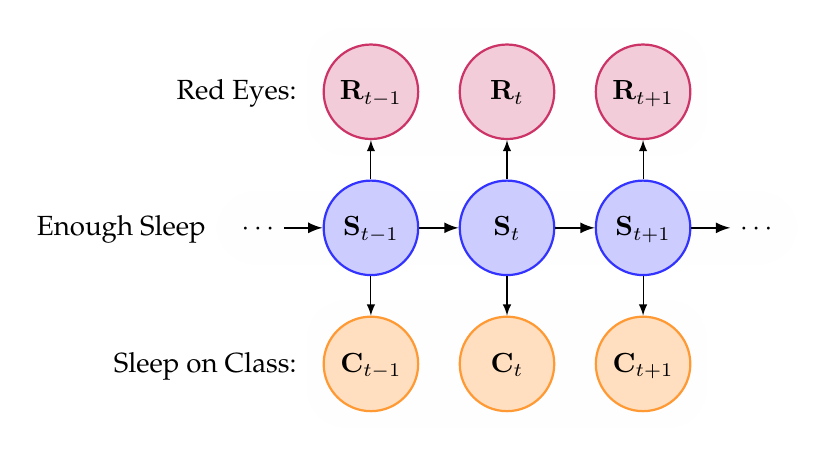
\begin{tikzpicture}[>=latex,text height=1.5ex,text depth=0.25ex]
	% "text height" and "text depth" are required to vertically
	% align the labels with and without indices.
	
	% The various elements are conveniently placed using a matrix:
	\matrix[row sep=0.5cm,column sep=0.5cm] {
		% First line: Control input
		&
		\node (u_k-1) [input]{$\mathbf{R}_{t-1}$}; &
		\node (u_k)   [input]{$\mathbf{R}_t$};     &
		\node (u_k+1) [input]{$\mathbf{R}_{t+1}$}; &
		\\
		% Third line: State & state transition matrix
		\node (A_k-2)         {$\cdots$};           &
		\node (x_k-1) [state] {$\mathbf{S}_{t-1}$}; &
		\node (x_k)   [state] {$\mathbf{S}_t$};     &
		\node (x_k+1) [state] {$\mathbf{S}_{t+1}$}; &
		\node (A_k+1)         {$\cdots$};           \\
		% Fifth line: Measurement
		&
		\node (z_k-1) [measurement] {$\mathbf{C}_{t-1}$}; &
		\node (z_k)   [measurement] {$\mathbf{C}_t$};     &
		\node (z_k+1) [measurement] {$\mathbf{C}_{t+1}$}; &
		\\
	};
	
	% The diagram elements are now connected through arrows:
	\path[->]
	(A_k-2) edge[thick] (x_k-1)	% The main path between the
	(x_k-1) edge[thick] (x_k)		% transition matrices is
	(x_k)   edge[thick] (x_k+1)	% x -> A -> x -> A -> ...
	(x_k+1) edge[thick] (A_k+1)
	
	(x_k-1) edge (u_k-1) 
	(x_k) edge (u_k)
	(x_k+1) edge (u_k+1)
	
	(x_k-1) edge (z_k-1)
	(x_k) edge (z_k) 
	(x_k+1) edge (z_k+1) 
	;
	
	% Now that the diagram has been drawn, background rectangles
	% can be fitted to its elements. This requires the TikZ
	% libraries "fit" and "background".
	% Control input and measurement are labeled. These labels have
	% not been translated to English as "Measurement" instead of
	% "Messung" would not look good due to it being too long a word.
	\begin{pgfonlayer}{background}
	\node [background2,
	fit=(u_k-1) (u_k+1),
	label=left:Red Eyes:] {};
	\node [background2,
	fit=(A_k-2) (A_k+1),
	label=left:Enough Sleep] {};
	\node [background2,
	fit=(z_k-1) (z_k+1),
	label=left:Sleep on Class:] {};
	\end{pgfonlayer}
	\end{tikzpicture}
	\quad 
	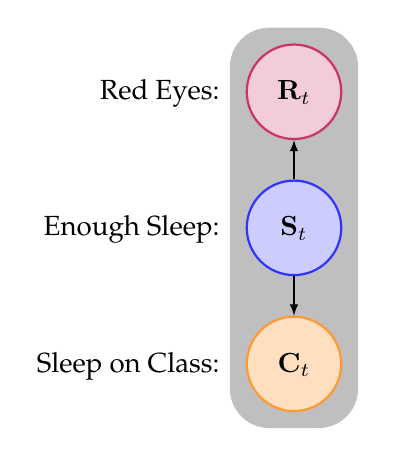
\begin{tikzpicture}[>=latex,text height=1.5ex,text depth=0.25ex]
		% "text height" and "text depth" are required to vertically
		% align the labels with and without indices.
		
		% The various elements are conveniently placed using a matrix:
		\matrix[row sep=0.5cm,column sep=0.5cm] {
			% First line: Control input
			\node (u_k)   [input]{$\mathbf{R}_t$};     &\\
			% Third line: State & state transition matrix
			\node (x_k)   [state] {$\mathbf{S}_t$};     &\\
			% Fifth line: Measurement
			\node (z_k)   [measurement] {$\mathbf{C}_t$};     &\\
		};
		
		% The diagram elements are now connected through arrows:
		\path[->]		
		(x_k) edge (u_k)
		
		(x_k) edge (z_k) 
		;
		
		% Now that the diagram has been drawn, background rectangles
		% can be fitted to its elements. This requires the TikZ
		% libraries "fit" and "background".
		% Control input and measurement are labeled. These labels have
		% not been translated to English as "Measurement" instead of
		% "Messung" would not look good due to it being too long a word.
		\begin{pgfonlayer}{background}
		\node [background2,
		fit=(u_k),
		label=left:Red Eyes:] {};
		\node [background2,
		fit=(x_k),
		label=left:Enough Sleep:] {};
		\node [background2,
		fit=(z_k),
		label=left:Sleep on Class:] {};
		\node [background,
		fit=(u_k) (z_k)] {};
		\end{pgfonlayer}
		\end{tikzpicture}
			
	\caption{Dynamic Bayesian Network. \textbf{Right}: Express by plate model} \label{fig:dbn}
\end{figure}

Model as Hidden Markov Model, ref to fig~\vref{fig:hmm}. The variable $R_t$ and $C_t$ is combined as $RC_t$. The conditional probability table becomes 
\begin{center}
\begin{tabular}{l|llll}
$RC_t=$ & $t,t$ & $t,f$ &$f,t$ & $f,f$ \\ \hline
$S_t=t$ &0.02&0.18&0.08&0.72 \\
$S_t=f$ &0.21&0.49&0.09&0.21 
\end{tabular}
\end{center}

\begin{figure}[htbp]
	\centering
	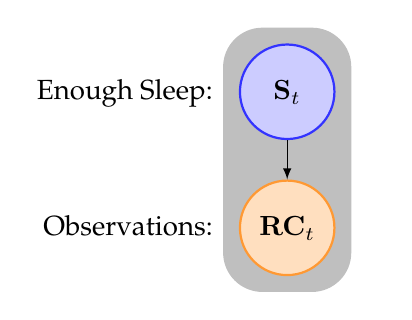
\begin{tikzpicture}[>=latex,text height=1.5ex,text depth=0.25ex]
	% "text height" and "text depth" are required to vertically
	% align the labels with and without indices.
	
	% The various elements are conveniently placed using a matrix:
	\matrix[row sep=0.5cm,column sep=0.5cm] {
		% Third line: State & state transition matrix
		\node (x_k)   [state] {$\mathbf{S}_t$};     &\\
		% Fifth line: Measurement
		\node (z_k)   [measurement] {$\mathbf{RC}_t$};     &\\
	};
	
	% The diagram elements are now connected through arrows:
	\path[->]		
	(x_k) edge (z_k) 
	;
	
	% Now that the diagram has been drawn, background rectangles
	% can be fitted to its elements. This requires the TikZ
	% libraries "fit" and "background".
	% Control input and measurement are labeled. These labels have
	% not been translated to English as "Measurement" instead of
	% "Messung" would not look good due to it being too long a word.
	\begin{pgfonlayer}{background}
	\node [background2,
	fit=(x_k),
	label=left:Enough Sleep:] {};
	\node [background2,
	fit=(z_k),
	label=left:Observations:] {};
	\node [background,
	fit=(x_k) (z_k)] {};
	\end{pgfonlayer}
	\end{tikzpicture}
	\caption{Hidden Markov Model, expressed by plate model} \label{fig:hmm}
\end{figure}

\section{Problem 4} 
\begin{description}
	\item[a.] Using frequency to estimate probability: 
	
	\begin{tabular}{c|c}
		$Y$ & $\mP(Y)$ \\ \hline
		-1 & 1/2 \\
		1 & 1/2 
	\end{tabular}  \quad
	\begin{tabular}{c|cc} 
		$X_1$ & $\mP(X_1|Y=-1)$ & $\mP(X_1|Y= 1)$ \\  \hline
		$0$& 1/3 &2/3\\
		$1 $& 2/3&1/3
	\end{tabular} \quad 
	\begin{tabular}{c|cc}
		$X_2$&$\mP(X_2|Y=-1)$ &$\mP(X_2|Y= 1)$ \\ \hline 
		0&2/3&2/3\\
		1&1/3&1/3
	\end{tabular}
	\item[b.] Add k (Laplace) smoothing, with $k=1$, 
	$${\mP(X_i|Y)}={\frac {N_{i}+k }{N+ k \times 2}}\qquad (i=1,2)$$
	\begin{tabular}{c|c}
		$Y$ & $\mP(Y)$ \\ \hline
		-1 & 1/2 \\
		1 & 1/2 
	\end{tabular}  \quad
	\begin{tabular}{c|cc} 
		$X_1$ & $\mP(X_1|Y=-1)$ & $\mP(X_1|Y= 1)$ \\  \hline
		$0$& 2/5 &3/5\\
		$1 $& 3/5&2/5
	\end{tabular} \quad 
	\begin{tabular}{c|cc}
		$X_2$&$\mP(X_2|Y=-1)$ &$\mP(X_2|Y= 1)$ \\ \hline 
		0&3/5&3/5\\
		1&2/5&2/5
	\end{tabular}
	\item[c.] $$\begin{array}{ll}
	 \mP(Y|X_1=0,X_2=0)& =\sfrac{\mP(Y,X_1=0,X_2=0)}{\mP(X_1=0,X_2=0)} \\
	& \propto \mP(Y)\mP(X_1=0|Y) \mP(X_2=0|Y) \\ 
	 & (\text{Since the evidence $\mP(X_1=0,X_2=0)$ is just a normalization factor} ) \\
	&=<\sfrac{1}{2}\times\sfrac{2}{5}\times\sfrac{3}{5},\sfrac{1}{2}\times\sfrac{3}{5}\times\sfrac{3}{5}> 
	\end{array}$$ 
	
	After normalization,  $\mP(Y|X_1=0,X_2=0)=<0.4,0.6>$. 
	\item[d.] When $k \rightarrow \infty $, the prior is dominant. $${\mP(X_i|Y)}=\lim_{k\rightarrow \infty} {\frac {N_{i}+k }{N+ k \times 2}}\qquad (i=1,2) =1/2 $$
	All value of table in {(b).} will be 1/2. Thus, $\mP(Y|X_1=0,X_2=0)=<0.5,0.5>$
	\item[e.] The following feature set can consist a linear binary classifier. 
	\begin{description}
		\item[v.] with decision boundary $abs(X_1-X_2)=1/2$
		\item[vii.] with decision boundary(not optimal) $2\max(X_1,X_2)-X_1-X_2=\epsilon, \text{where } \epsilon \rightarrow 0^{+}$
		\item[viii.] with decision boundary $I(X_1-X_2)=1/2$
	\end{description}
\end{description}

\section{Problem 5}
In space of ${X_1, X_1X_2}$, the margin is $X_1X_2=0$, draw the separating line back to origin Euclidean input space, there are two lines $X_1=0$ and $X_2=0$.

\includegraphics[width=.48\columnwidth]{1.png}
\includegraphics[width=.5\columnwidth]{2.png}
%\begin{thebibliography}{99}
%\bibitem{1} Silver, David, et al. "Mastering the game of Go with deep neural networks and tree search." Nature 529.7587 (2016): 484-489.
%Publishing Company , 1984-1986.
%\bibitem{2} \url{https://www.quora.com/Are-neural-networks-the-future-of-AI}
%\bibitem{3} \url{https://youtu.be/yCALyQRN3hw?list=PLqYmG7hTraZA7v9Hpbps0QNmJC4L1NE3S&t=11434}
%
%\end{thebibliography}	
	
\end{document}
